%add
\section{Hydraulic structures}
\label{sec-structures}
The term {\em hydraulic structures} refers to control structures such as tidally-operated gates, 
barriers, weirs and culverts as well as to coupled boundary conditions 
representing direct transfers of water from an outflow to an inflow boundary due to mechanisms like low head pumps. 
There are numerous gates and control structures in the San Francisco Bay-Delta. Here we describe the way structures are modeled and the formulas used to calculate flow through them. 

Hydraulic structures are represented in SCHISM as paired boundary condition (Figure \ref{fig:structmesh}). Flow is calculated based on head differences at two {\em reference nodes}, one on the nominal upstream and downstream sides of the structure (but not necessarily adjoining the structure). Once the flow is calculated, it is disaggregated as a homogenous flux boundary condition over the breadth of the structure. The boundaries are enforced using a relaxation formulation, which provides some natural ramping of flow when gates that are suddenly opened or closed. Transport is coupled between the side that is an outflow and the side that is an inflow.

\begin{figure}
	\centering
		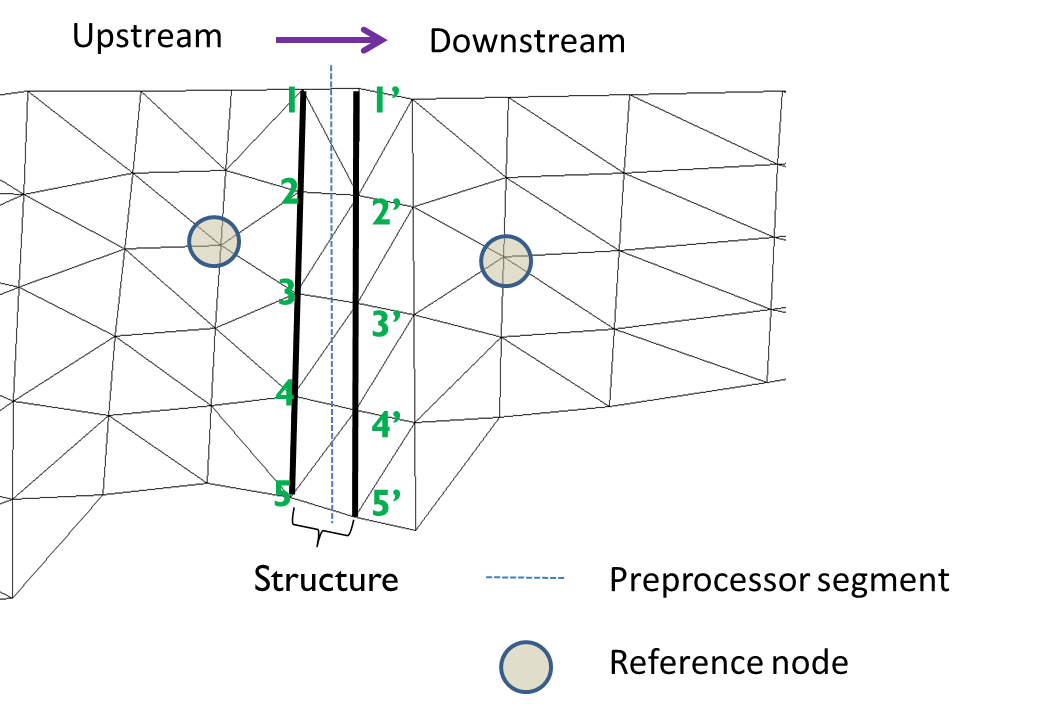
\includegraphics[scale=1]{image/struct}
	\caption{Hydraulic structure definition imposed on horizontal grid.}
	\label{fig:structmesh}
\end{figure}

A number of pre-defined flow structures are already in place covering all the cases we encountered in the Bay-Delta; with a little programming the system can easily be expanded to accommodate new structures.  
The structures we have already implemented are listed below. All of the structures admit control of key (indicated) parameters using time series. 

Structures can also be removed in SCHISM by adding 
an appropriate entry in a time series. When a structure is removed, the region between the paired boundaries reverts to the ordinary equations of motion -- ie, it is if the structure did not exist.

\subsection{Flow transfers}
\label{sec-transfer}
A flow transfer is a simple coupled boundary condition wherein a fixed flow $Q_s$ is stipulated. This flow
is imposed as an outflow boundary on one the paired boundaries and and inflow on the other. Constituent mass 
is conserved.

\begin{figure}
	\centering
		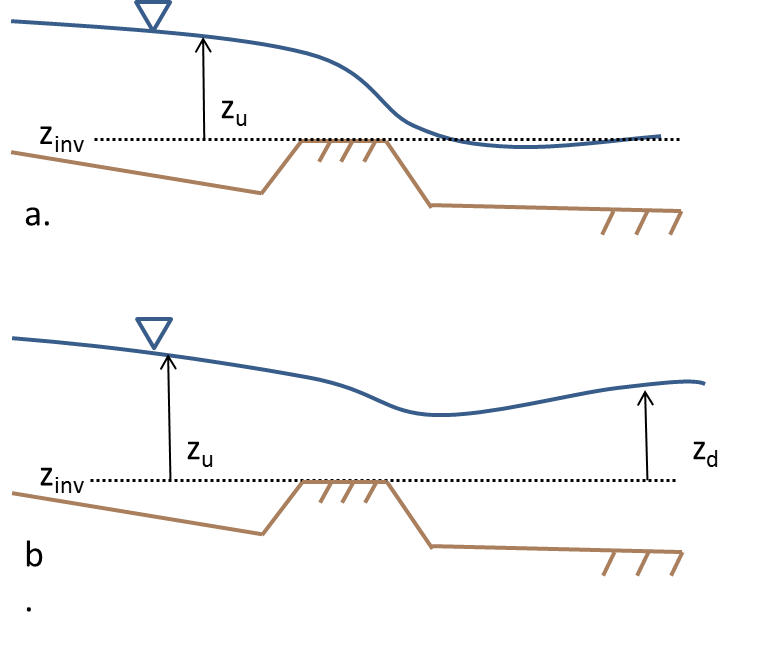
\includegraphics[scale=1]{image/weir}
	\caption{Free flowing (a) and submerged (b) weir flow cases.}
	\label{fig:weir}
\end{figure}

\subsection{Weirs}
A weir may be dry, submerged or free flowing (see Figure \ref{fig:weir}) depending on the position of the upstream
and downstream water surfaces $z_{u}$, $z_{d}$ compared to the weir invert elevation $z_{inv}$. Note that in the formulas
below, 

For the free flowing case:
$$
Q_s^f=\sgn{(z_{u} - z_{d})} C_{op} C_{f} A \sqrt{2g H}
$$
where 
\begin{align*}
&Q_s^f  &\text{free flow flow through structure (cms)} &\\
&\sgn        &\text{sign function (to induce up/downstream directionality)}  &\\
&z_u         &\text{upstream reference elevation  (m)}  &\\
&z_d         &\text{downstream reference elevation (m)}  &\\
&z_{inv}     &\text{invert elevation of the weir (m)}  &\\
&H = \max(z_u,z_d) - z_{inv}  &\text{is the energy head above the weir} &\\
&A                            &\text{area of flow (m\textsuperscript{2}) }&\\
&C_op               &\text{(directionally varying) operating coefficient (unitless)} &\\
&C_f                &\text{flow/gate coefficient (unitless)}  &\\
&g                  & \text{gravity (m/s\textsuperscript{2})} & \\
\end{align*}
For commentary on coefficients, see \cite{Rantz82}. Note that in the formulation above, the $\sqrt{2g}$
term has been kept separate and the area calculation uses water surface height. 
Furthermore, note that $z_u$ and $z_d$ are pre-assigned upstream and downstream orientations,
whereas $H$ is the energy head in the direction that is upstream of the weir in terms of actual flow.

The submerged case is derived from the free flowing case using the correction given by \citet{Villemonte47}:
\begin{align*}
Q_s^s = Q_s^f(1 - S^{1.5})^{0.385} \\
S = \frac{\min(z_u,z_d) - z_{inv}}{\max(z_u,z_d) - z_{inv}}
\end{align*}
in terms of the {\em submergence ratio} $S$.

If both sides are dry, of course $Q_s=0$ for the structure. Note that this refers to being dry with respect to the invert elevation.
The nodes may not go dry in the ordinary sense with respect to the bed -- this is the same restriction as at other SCHISM boundaries. 

\subsection{Radial gates} 
\label{sec:radial}
A radial gate is parametrized as shown in Figure \ref{fig:radial}, although at the moment we have ignored the kinetic 
energy component of upstream head (so that $H_1 = y_1$). For the case where the radial gate is completely out
of the water or the tailwater elevation is not sufficiently high to affect the upstream (submergence ratio described in the previous
section is less than $S_p=0.66$),
the gate reverts to a modified weir equation described momentarily. For the case where the radial gate is completely submerged 
(submergence ratio greater than $S_f=0.80$),
the gate is treated as an orifice as given in Section \ref{sec-orifice}.

            %diff = max_elev - min_elev
            %coef_matching_factor = sqrt(1.d0/(1.d0-PART_SUBMERGE))
            %flow = signed_coef*area*sqrt2g*sqrt(diff)
            %! now weigh the two so that the flow makes a linear transition
            %subfrac = (submerge_ratio-PART_SUBMERGE)/(FULL_SUBMERGE - PART_SUBMERGE)
            %flow = ((1.d0 - subfrac)*coef_matching_factor + subfrac)*flow
For free flow:
$$
Q_s^f = \sgn{(z_{u} - z_{d})} C_{op} C_{f} A \sqrt{2g H}
$$
and for partially submerged flow ($S_p < S \le S_f$):
$$
Q_s^p = \sgn{(z_{u} - z_{d})} C_{op} C_{f} A \sqrt{2g \left|\D z\right|}[(1-\hat{S})m+\hat{S}]
$$
where
\begin{align*}
&\hat{S}=\frac{S-S_p}{S_f-S_p} & \text{is the submergence fraction} \\
&m = \sqrt{\frac{1}{1-S_p}} & \text{is a coefficient matching factor to create a smooth transition}. \\
\end{align*}

For fully submerged flow $S>S_f$, the orifice equation is used. This is equivalent to the submerged equation with
$\hat{S}=1$.


\begin{figure}
	\centering
		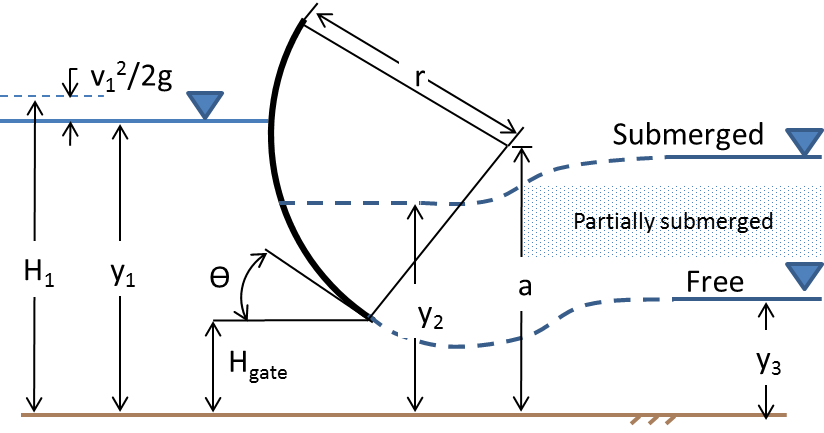
\includegraphics[scale=1]{image/radial_gate}
	\caption{Radial gate.}
	\label{fig:radial}
\end{figure}

\subsection{Radial gates with linear coefficient} 
This is an alternative radial gate formula modified from a suggestion by Tony Wahl of the USBR (personal communication) 
that was incorporated because it matches Clifton Court well. 
The rating formula is a little simpler, but the flow coefficient is a linear function of gate height:

$$
Q_s = \sgn{(z_{u} - z_{d})} C_{op} C_{f} A \sqrt{2g \left|\D z\right|}
$$
where
$$C_f = d + sR$$
is the gate coefficient linearly dependent on the ratio of gate opening to upstream head:
$$R = \min(\frac{H_{gate}}{H_1},1.0)$$
with constant and linear parameters $d$ and $s$ respectively.
Some special cases surround the term $A$, given that the top of the radial gate
may be dry or submerged.

\subsection{Orifice}
\label{sec-orifice}
The orifice option is used to model a sluice gate or flashboard or other devices that  
presents a (rectangular) apertures to flow. Flow in this case is given by:

$$
Q_{s} = \sgn{(z_{u} - z_{d})} C_{op} C_{f} A \sqrt{2g \left|\D z \right|}
$$

Some special cases surround the term $A$, given that the orifice may be dry, partially submerged or completely
submerged. Typically, the orifice equation is most useful when flow is fully submerged.

\subsection{Culverts}
A culvert is currently modeled as a circular orifice. In other words, it is the same as the orifice case
but with a different formula for $A$. This treatment neglects some of the nuances of head and tailwater control 
as described by \cite{Bodhaine68}
